\documentclass{article}
\usepackage{graphicx} % Required for inserting images
\usepackage{tabularx,lipsum,environ,amsmath,amssymb}
\usepackage{algorithm}
\usepackage{algpseudocode}
\usepackage{placeins}
\usepackage{xcolor}
\usepackage{amsthm}

\usepackage{float}

\usepackage[a4paper, total={7in, 8in}]{geometry}

\makeatletter

\newtheorem{theorem}{Theorem}
\newtheorem{lemma}{Lemma}

\newenvironment{hashtable}[1][]
  {\begin{tabular}[#1]{
     @{} 
     > {\small} r <{\normalsize~\rlap{\fbox{\strut~~}}$~~\rightarrow$~}
     @{} l @{}}}
  {\end{tabular}}
 

\newcommand{\problemtitle}[1]{\gdef\@problemtitle{#1}}% Store problem title
\newcommand{\probleminput}[1]{\gdef\@probleminput{#1}}% Store problem input
\newcommand{\problemquestion}[1]{\gdef\@problemquestion{#1}}% Store problem question
\NewEnviron{problem}{
  \problemtitle{}\probleminput{}\problemquestion{}% Default input is empty
  \BODY% Parse input
  \par\addvspace{.5\baselineskip}
  \noindent
  \begin{tabularx}{\textwidth}{@{\hspace{\parindent}} l X c}
    \multicolumn{2}{@{\hspace{\parindent}}l}{\@problemtitle} \\% Title
    \textbf{Input:} & \@probleminput \\% Input
    \textbf{Problem:} & \@problemquestion% Question
  \end{tabularx}
  \par\addvspace{.5\baselineskip}
}
\makeatother

\newcommand{\ml}[1]{\begingroup\color{blue}#1\endgroup}
\newcommand{\rk}[1]{\begingroup\color{red}#1\endgroup}

\title{Finding segmental duplications and losses}
%\author{r3za.kalhor }
\date{}

\begin{document}

This document summarizes some results from the simphy simulations, with a WGD forced into its species tree.  There were $\sim$100 runs, each with $\sim$100 gene trees and species trees with $50$ leaves (to be confirmed).

The figure below shows the sum, over every gene tree evaluated, of the species  path distance (error) compared to the simulated simphy gene tree.
Here, $dx$ means the output from the greedy algorithm when $dup\_height\_cost = x$ and $loss\_cost = 1$.

\begin{figure}[H]
    \centering
    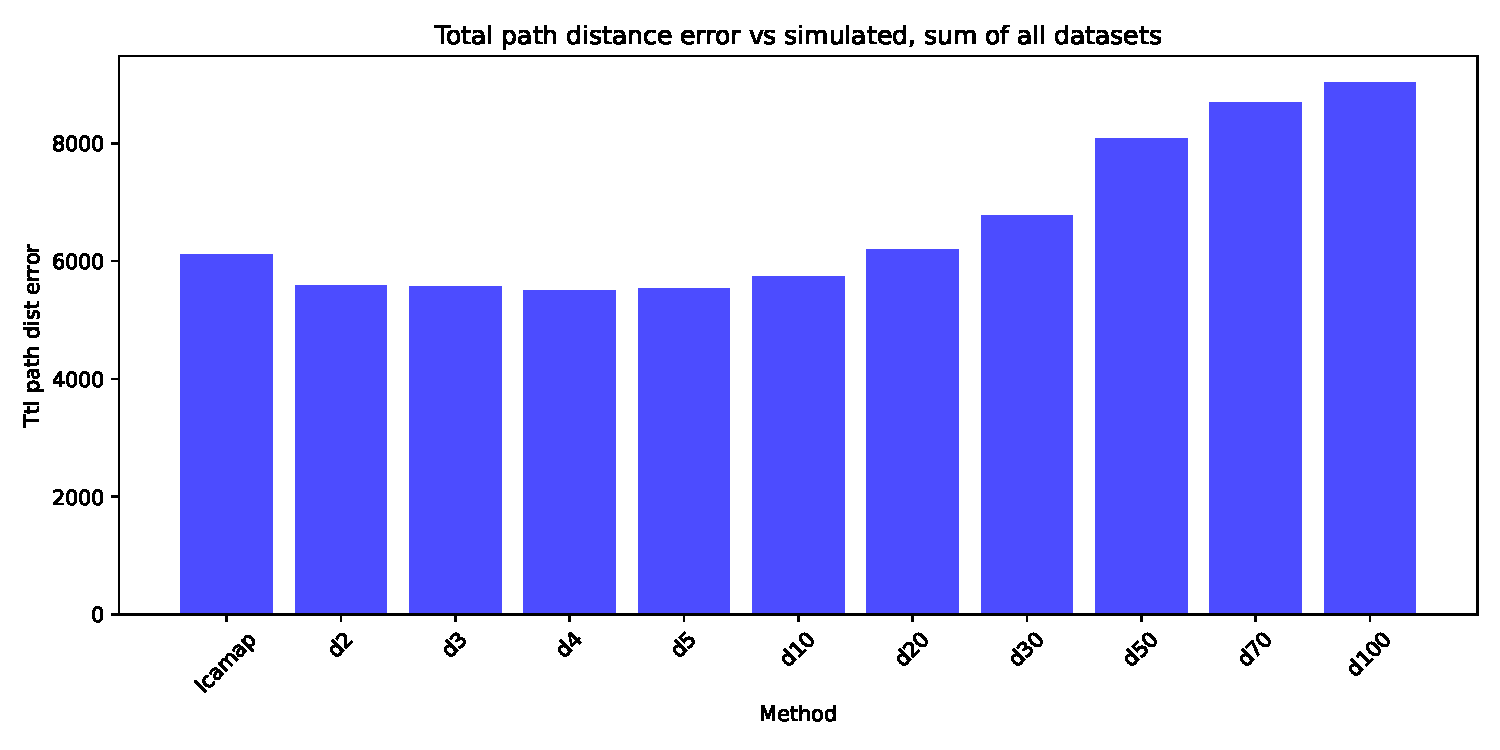
\includegraphics[width=\textwidth]{plots/dists.pdf}
    \caption{Sum of path distances (error) vs true simulated trees.  }
    \label{fig:enter-label}
\end{figure}

The improvements on small $d$ are not revolutionary, and allowing duplications to go too high creates more error.


\clearpage


Of course, we could also manipulate the visuals to tell a better story, as people do.  Here's the same plot, without $d50, d70, d100$, and the $y$ axis that starts around 5000.
Feels like cheating at this point, though.

\begin{figure}[H]
    \centering
    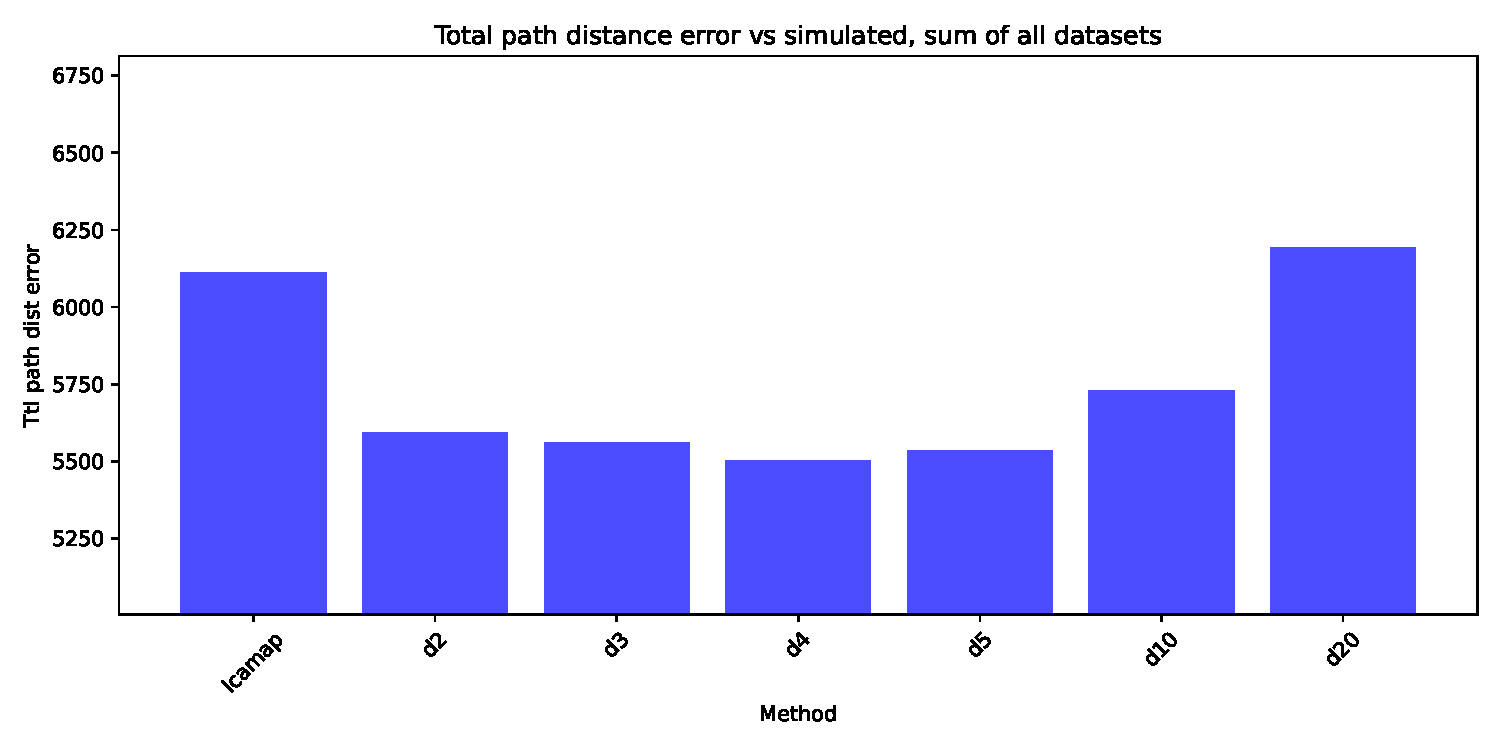
\includegraphics[width=\textwidth]{plots/dists_cheating.pdf}
    \caption{Sum of path distances (error) vs true simulated trees.  }
    \label{fig:enter-label}
\end{figure}




\clearpage 


How to read figure below: a simphy run is a simulation of one species tree and $m$ gene trees ($m = 100$?).  

In each run, we compute the path distance error  of lca summed over the $m$ gene trees, and we do the same for the greedy output.  

The improvement $\%$ is 
\[
1 - \frac{\mbox{greedy error}}{\mbox{lca error}}
\]
For instance, if lca makes 100 errors and greedy make 25, the improvement is $75\%$.
The plot shows the average error, taken across all simphy runs.
This value can be negative (even infinitely negative).

How to interpret: I don't know.  From the previous plot, $d30$ has a worse total error, but on average has a good improvement.  I guess it is more aggressive: when it improves, it improves by a high percentage, but overall it gets it wrong more often.

\begin{figure}[H]
    \centering
    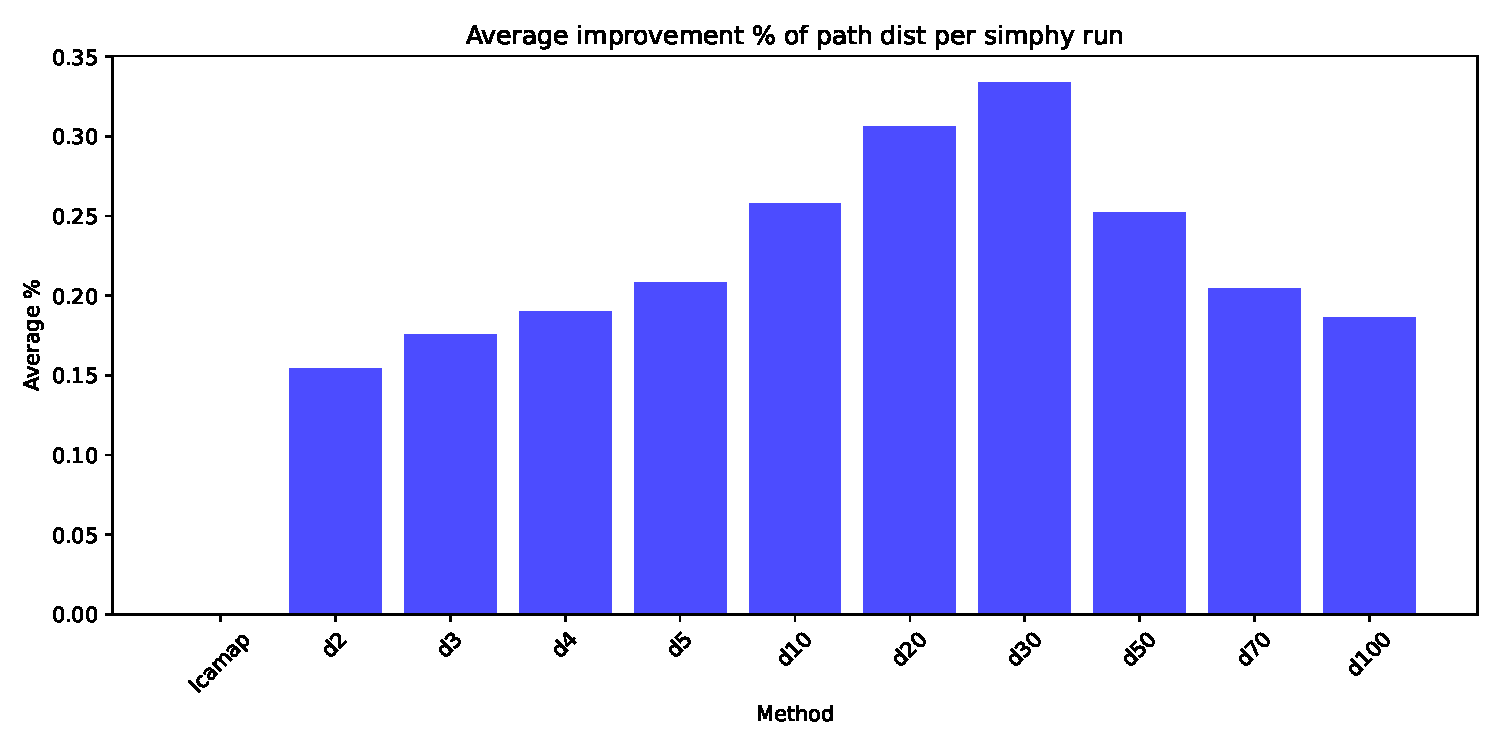
\includegraphics[width=\textwidth]{plots/avgpctimprov.pdf}
    \caption{Average improvement in path distance.  }
    \label{fig:enter-label}
\end{figure}



\clearpage



How to read this: this is just a summary of the first plot.  Instead of averaging per dataset, it just does
\[
1 - \frac{\mbox{final sum of greedy error}}{\mbox{final sum of lca error}}
\]
Since in Fig 1 d30 has more error than lca, this will be negative from d30 and onwards.


\begin{figure}[H]
    \centering
    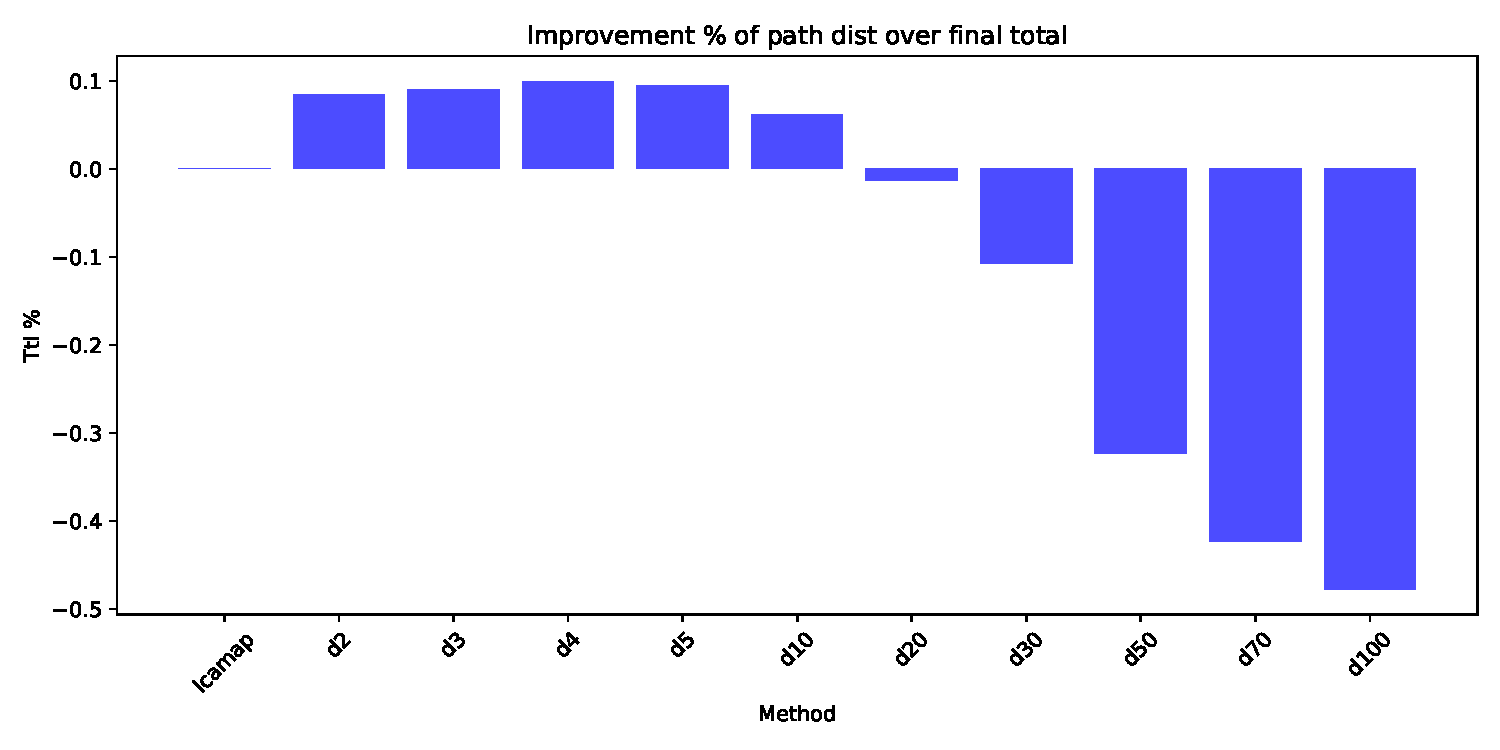
\includegraphics[width=\textwidth]{plots/pctimprov.pdf}
    \caption{Improvement percentage in final path distance.  }
    \label{fig:enter-label}
\end{figure}

\clearpage 



\begin{figure}[H]
    \centering
    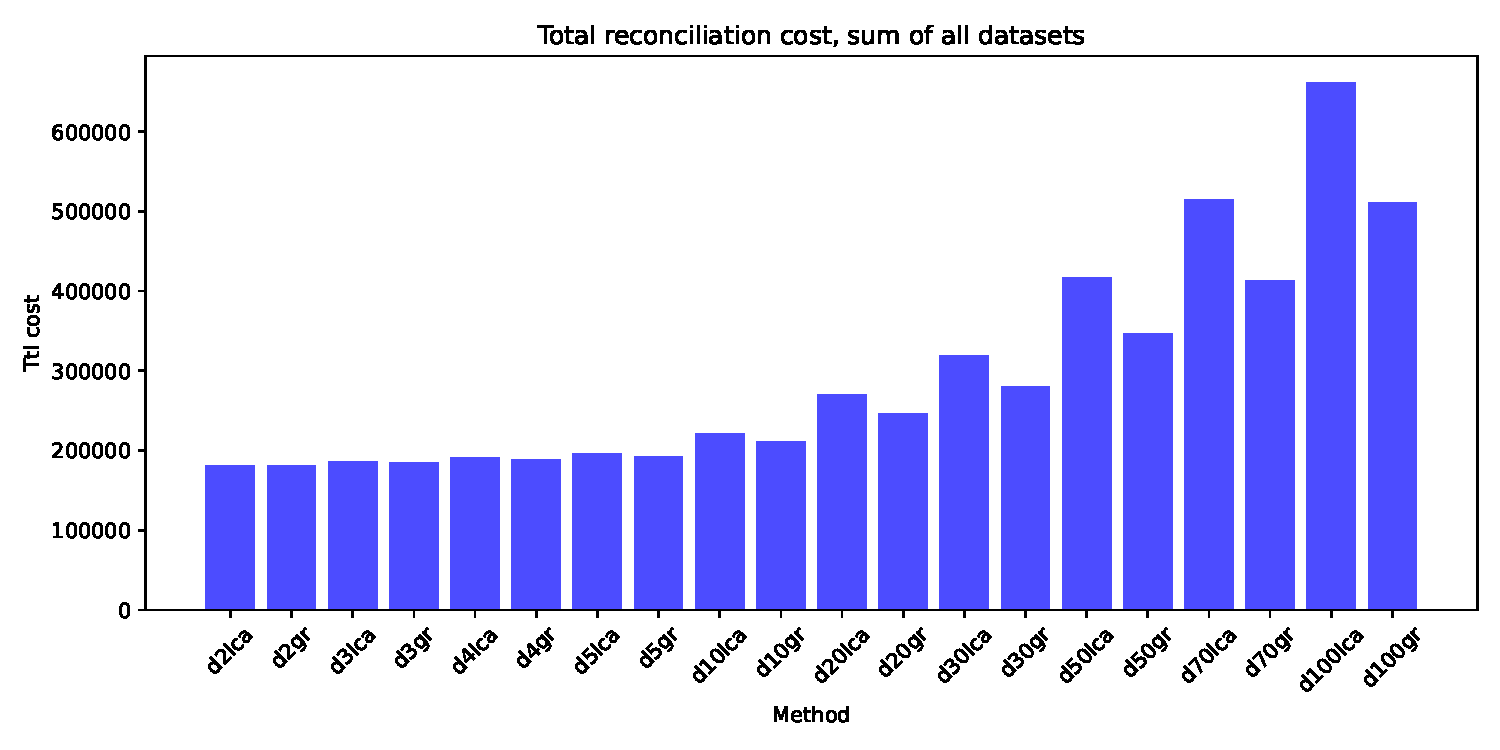
\includegraphics[width=\textwidth]{plots/costs.pdf}
    \caption{Sum of reconciliation costs, across all simphy datasets considered.  }
    \label{fig:enter-label}
\end{figure}


How to read this: $dxlca$ means the sum of reconciliation costs of the lca mapping, if $dup\_height\_cost=x$ and $loss\_cost = 1$.  Likewise, $dxgr$ is the sum of reconciliation costs produced by the greedy algorithm if the dup height cost is $x$.  For example, $d20gr$ is the output sum-of-costs from the greedy algorithm, with a cost one $20$ per segmental duplication, and a cost of $1$ per loss.

These should be read pair-by-pair, i.e., compare d2lca vs d2gr, because the lca cost is recalculated each time with respect to $d$.

Obviously, higher $d$ allow more moves and thus more potential for reduction in cost.


\clearpage 


\section*{Introducing fractionation}

In the following, we simulated fractionation as follows: for each gene tree $G$ and each leaf $l$ of $G$ (visited in a random order), let $k$ be the number of extant genes in the same species as $l$.  Then delete $l$ with probability $(k-1)/k$ (or something similar, then update $k$ for the next gene). 

The plots are similar.

\begin{figure}[H]
    \centering
    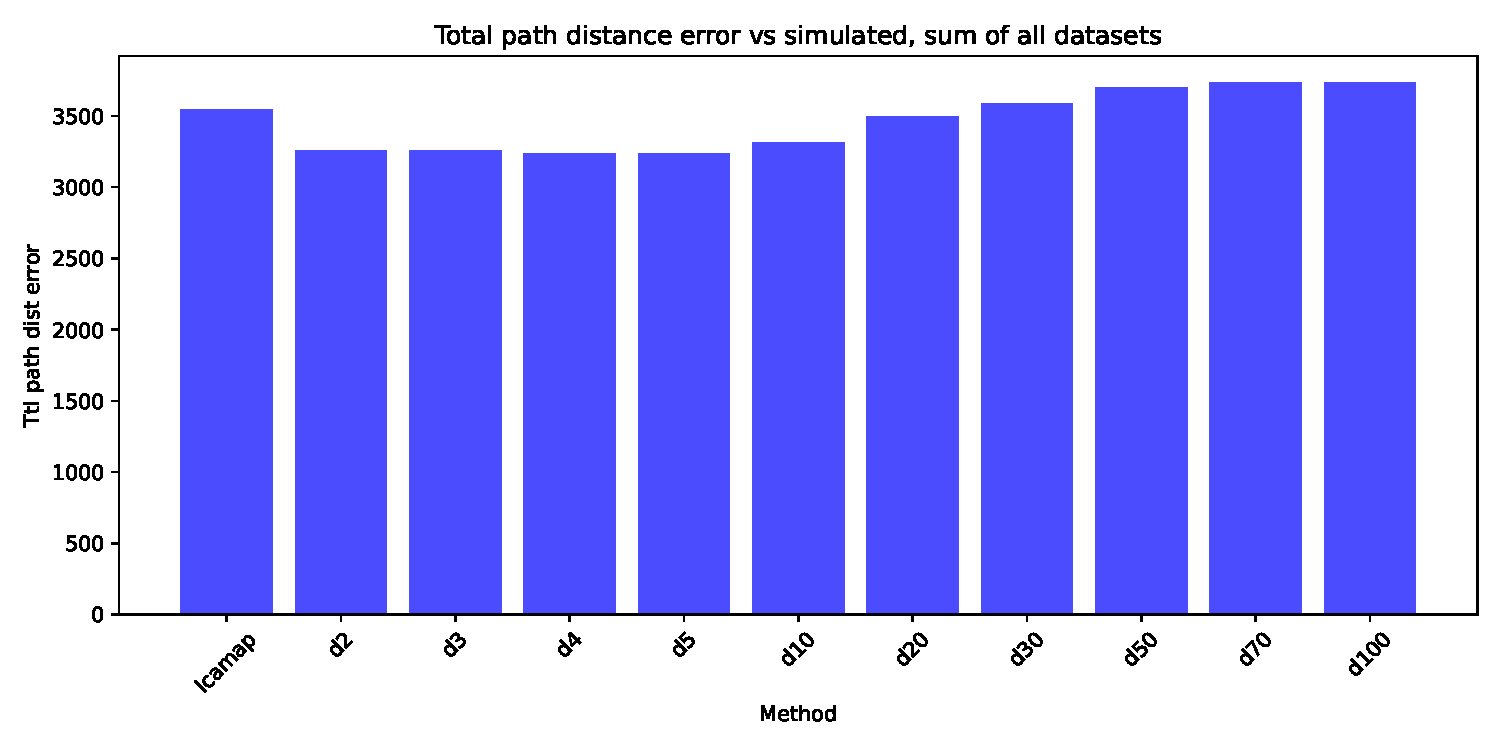
\includegraphics[width=\textwidth]{plots/dists_loss.pdf}
    \caption{Caption}
    \label{fig:enter-label}
\end{figure}

\begin{figure}
    \centering
    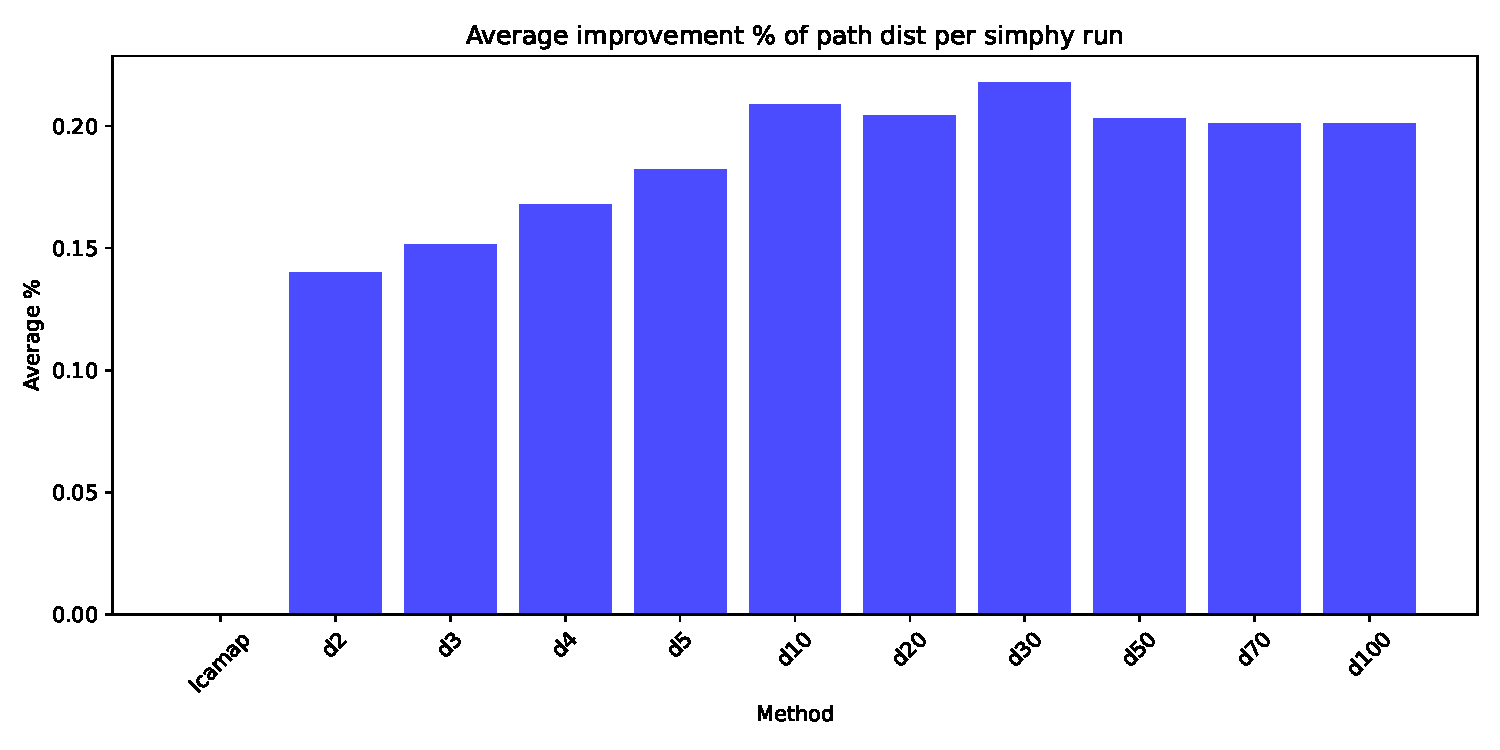
\includegraphics[width=\textwidth]{plots/avgpctimprov_loss.pdf}
    \caption{Caption}
    \label{fig:enter-label}
\end{figure}



\begin{figure}
    \centering
    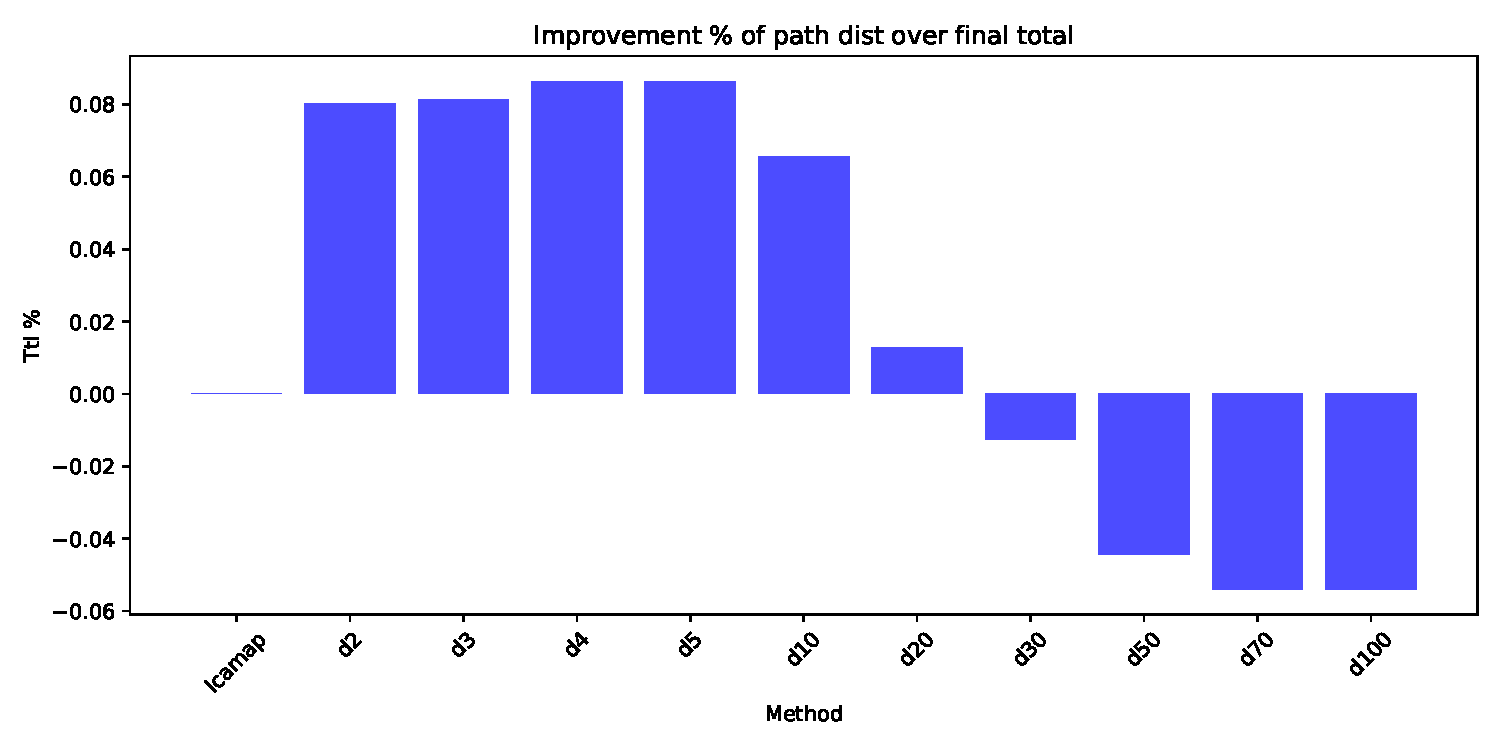
\includegraphics[width=\textwidth]{plots/pctimprov_loss.pdf}
    \caption{Caption}
    \label{fig:enter-label}
\end{figure}



\begin{figure}
    \centering
    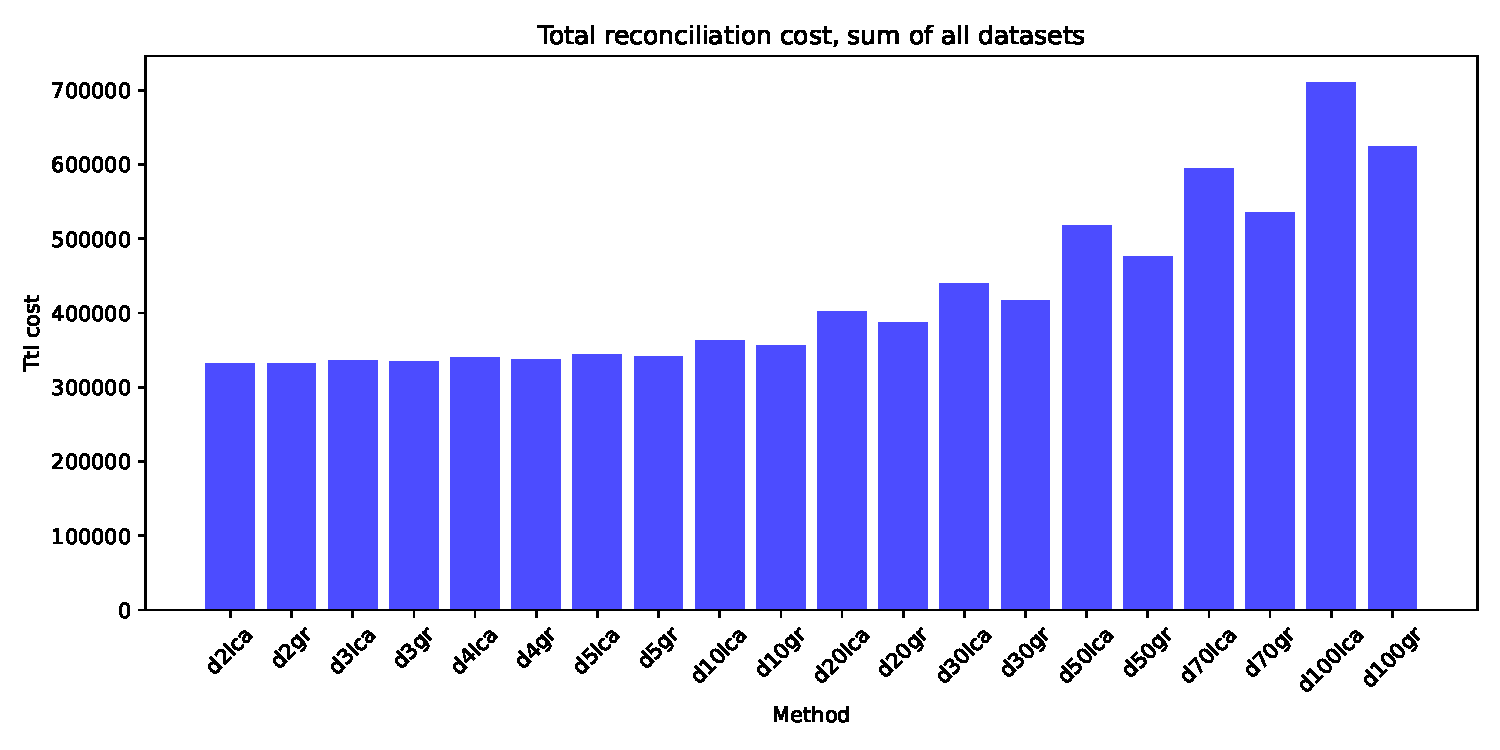
\includegraphics[width=\textwidth]{plots/costs_loss.pdf}
    \caption{Caption}
    \label{fig:enter-label}
\end{figure}


\clearpage

\section*{Dup rate = loss rate = 0 (only WGD)}

Here are the plots when the dup rate = loss rate = 0 in simphy.  So, only the WGD is present.

\begin{figure}[H]
    \centering
    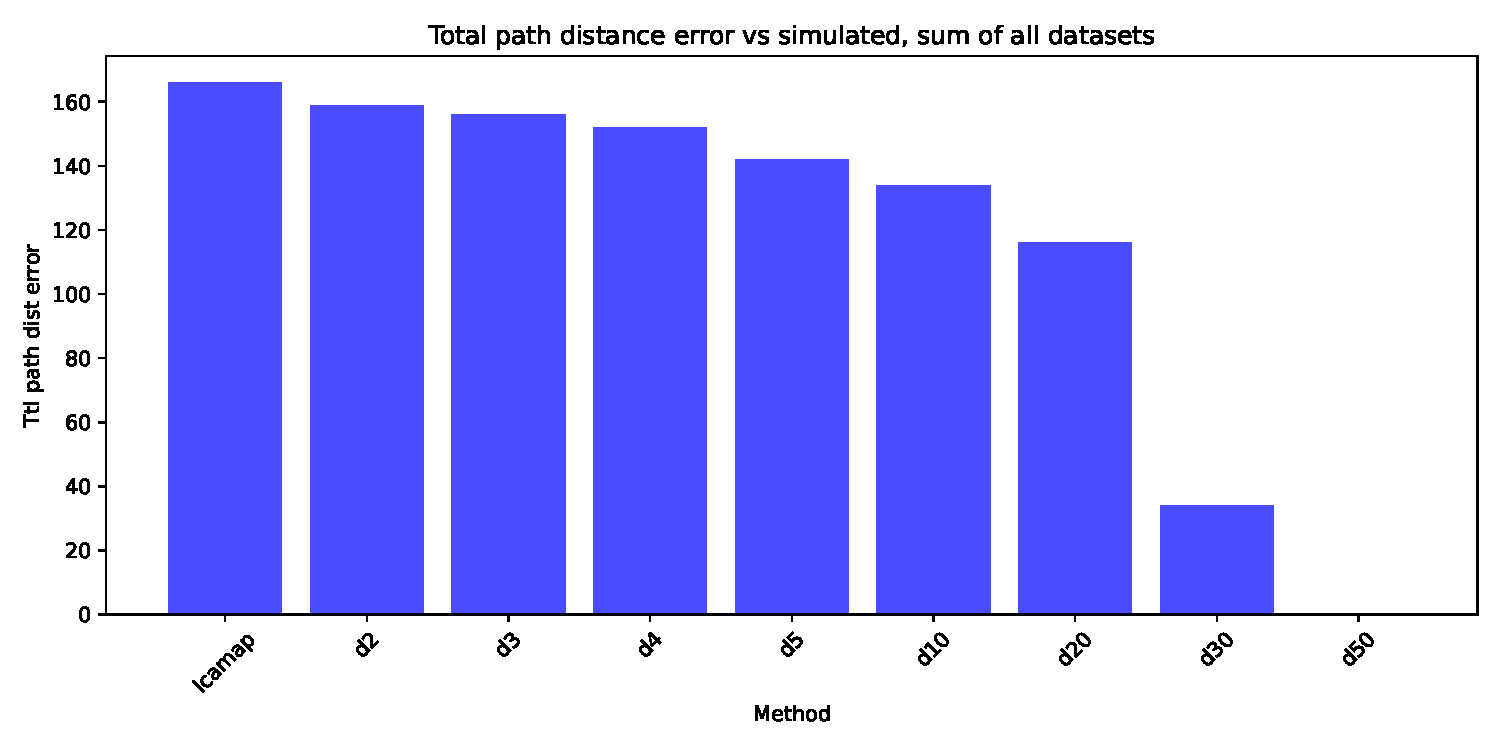
\includegraphics[width=\textwidth]{plots/dists_duprate0.pdf}
    \caption{Caption}
    \label{fig:enter-label}
\end{figure}


\begin{figure}
    \centering
    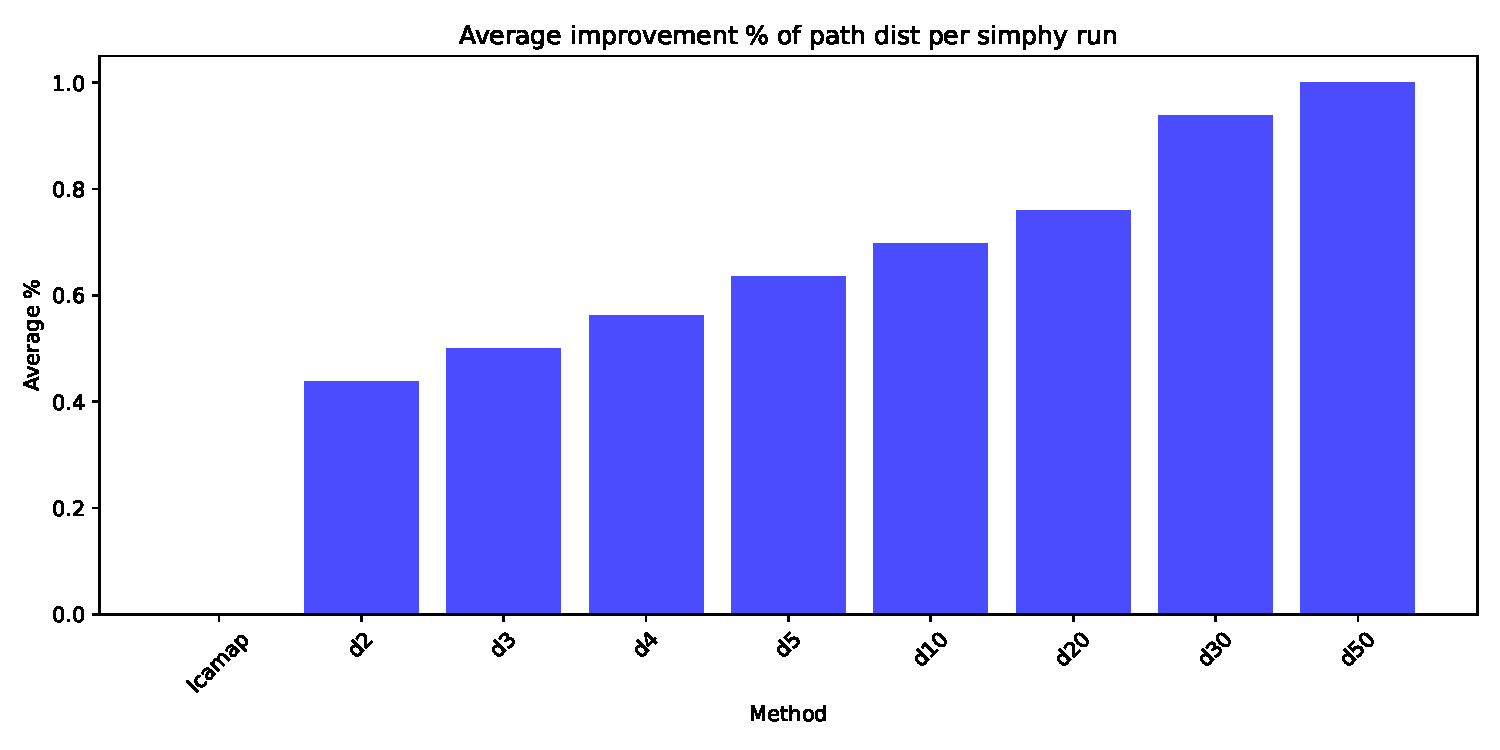
\includegraphics[width=\textwidth]{plots/avgpctimprov_duprate0.pdf}
    \caption{Caption}
    \label{fig:enter-label}
\end{figure}


\begin{figure}
    \centering
    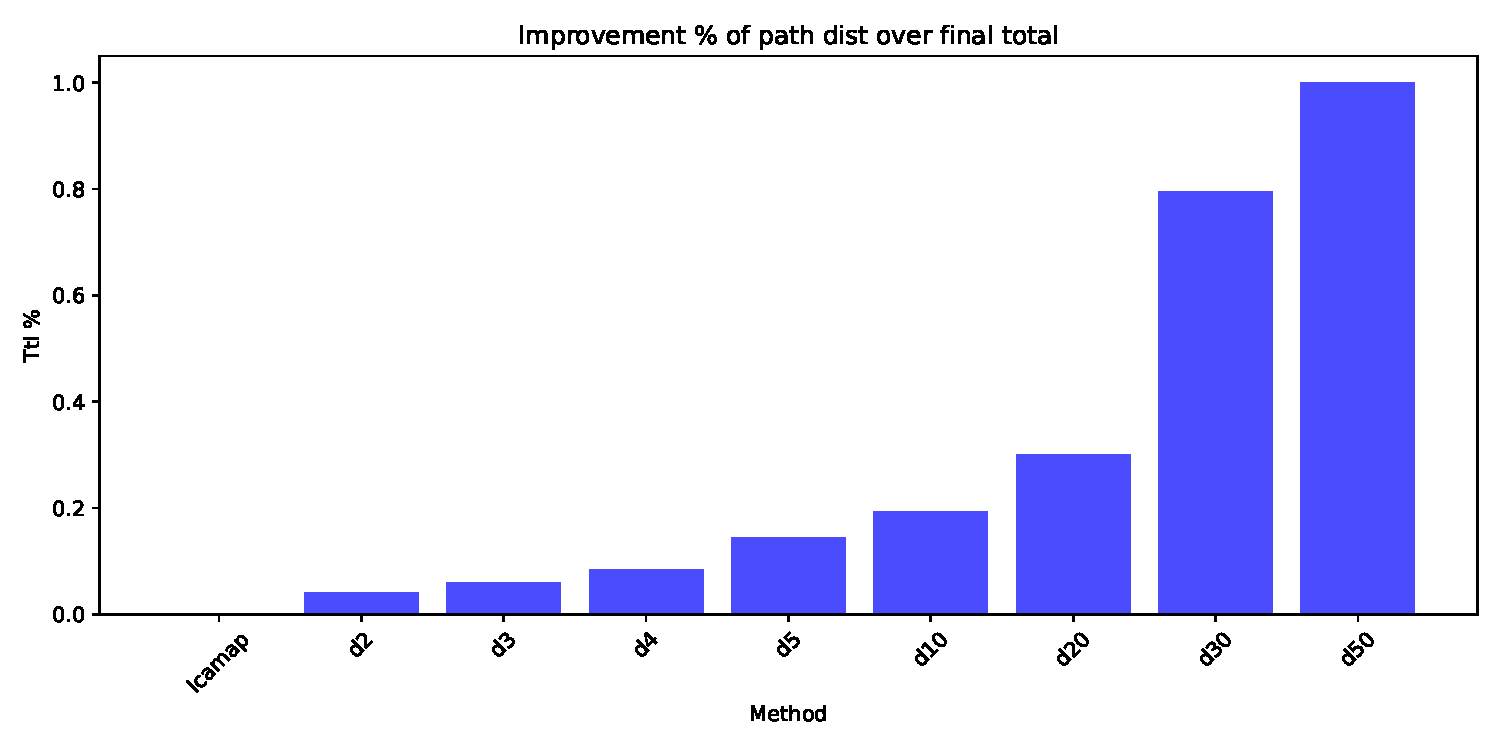
\includegraphics[width=\textwidth]{plots/pctimprov_duprate0.pdf}
    \caption{Caption}
    \label{fig:enter-label}
\end{figure}



\begin{figure}
    \centering
    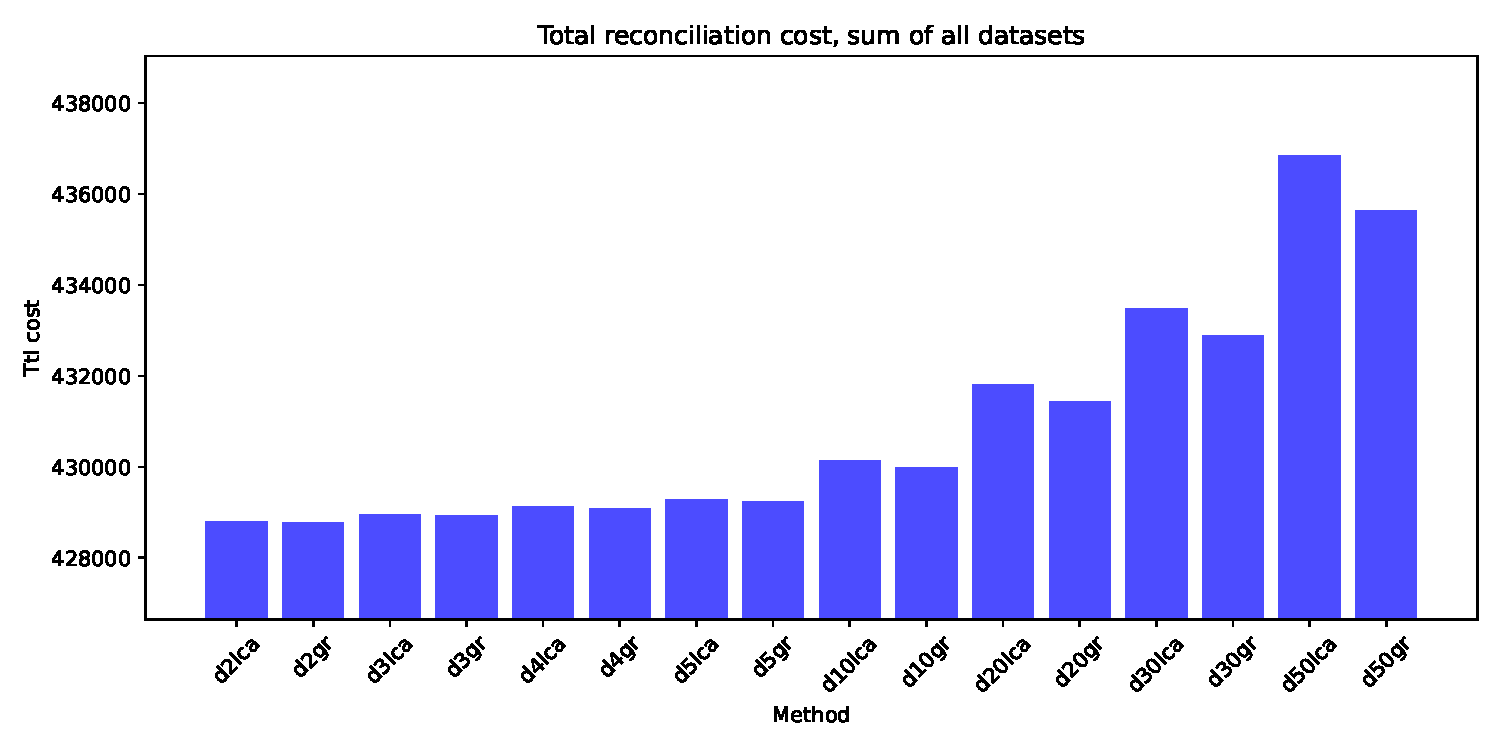
\includegraphics[width=\textwidth]{plots/costs_duprate0.pdf}
    \caption{Caption}
    \label{fig:enter-label}
\end{figure}



\end{document}
